\documentclass[12pt,a4paper]{report}
\usepackage[utf8]{inputenc}
\usepackage{amsmath}
\usepackage{amsfonts}
\usepackage{amssymb}
\usepackage{makeidx}
\usepackage{graphicx}
\usepackage{cancel}
\author{Marius Ketterer}
\title{Praktikum Regelungstechnik 2 Abgabe Versuch 1 Digitale Übertragungsglieder}
\begin{document}

\maketitle
\tableofcontents

\chapter{Tiefpass 1.Ordnung}
\section{Aufstellen der Übertragungsfunktionen im s-Bereich inklusive Halteglied}
Aufstellen der Übertagungsfunktionen
\begin{equation}
G_{PT1}(s) = \frac{K}{1-Ts} 
\end{equation}
\begin{equation}
H(s) = \frac{1-e^{T_As}}{s}
\end{equation}
Transformieren in den Z-Bereich
\begin{equation}
G(z) = \mathcal{Z}\{H(s)*G_{PT1}(s)\} = \mathcal{Z}\left\{\frac{1-e^{T_As}* G(s)}{s}\right\}
\end{equation}

\begin{equation}
G(z) = \mathcal{Z}\left\{1-e^{T_As}*\frac{G(s)}{s}\right\} = (1-z^{-1})*\mathcal{Z}\left\{\frac{K}{s(1+Ts)}\right\}
\end{equation}

\begin{equation}
G(z) = (1-z^{-1})*\mathcal{Z}\left\{K\frac{\frac{1}{T}}{s(\frac{1}{T}+s)}\right\}
\end{equation}
Transformieren mit Hilfe der Korrespondenzentabelle(Nr.8)
\begin{equation}
G(z) = K*\cancel{(1-z^{-1})}*
\frac{(1-e^{-\frac{T_A}{T}})z^{-1}}
{\cancel{(1-z^{-1})}(1-e^{-\frac{T_A}{T}}z^{-1})}
\end{equation}
Daraus ergibt sich: 
\begin{equation}
G(z) = \frac{K*z^{-1}-e^{-\frac{T_A}{T}}z^{-1}}
{1-e^{-\frac{T_A}{T}}z^{-1}} 
\end{equation}
Einsetzen der Werte
\begin{equation}
K = 3; T = 4; T_A = 0,5s
\end{equation}
\begin{equation}
G(z) = \frac{3z^{-1}-e^{-\frac{0,5}{4}}z^{-1}}
{1-e^{-\frac{0,5}{4}}z^{-1}} = \frac{2,118z^{-1}}{1-0,882z^{-1}} = \frac{Y}{X}
\end{equation}
\begin{equation}
 Y- 0,882z^{-1}Y = 2,118z^{-1}X
\end{equation}
Nach $ Y $ aufgelöst ergibt das:
\begin{equation}
\Rightarrow Y = 2,118z^{-1}X - 0,882z^{-1}Y
\end{equation}
\begin{figure}
\centering
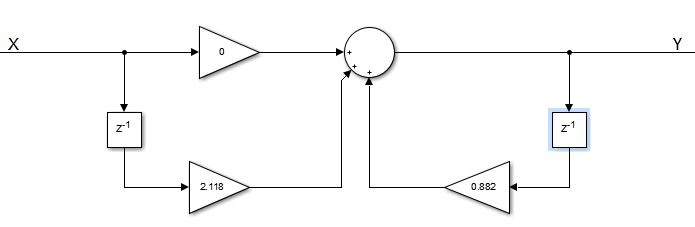
\includegraphics[width=0.7\linewidth]{marius/PT1}
\caption{}
\label{fig:PT1}

\end{figure}

	
\end{document}